% !TEX root = calculus.tex


\chapter{VELOCITY}
\label{velocity}
{\parindent=0pt

\athr We are practically ready to tackle the concept of a \emph{derivative}. This concept, alongside with the concepts of the \emph{limit of numerical sequence} and the \emph{limit of function}, is one of the most important special concepts in calculus.

We may approach the concept of a derivative by considering, for instance, a quantity widely used in physics: the \emph{instantaneous velocity} of nonuniform motion of a body.

\rdr We have been familiarized with this notion when studying kinematics in the course of physics, or, to be precise, the kinematics of nonuniform motion in a straight line.

\athr Exactly. What is your idea of the instantaneous velocity?

\rdr The instantaneous velocity of a body is defined as the velocity of a body at a given moment of time (at a given point of its trajectory).

\athr And what is your idea of the \emph{velocity at a given moment of time}?

\rdr Well, I see it as \ldots If a body moves uniformly, at different moments of time its velocity remains the same. If a body moves non-uniformly (accelerating or decelerating), its velocity will, in the general case, vary from moment to moment.

\athr Don't you feel that the phrase ``velocity at a given moment of time'' is merely a \emph{paraphraze} of the ``instantaneous velocity''? Six of one and half a dozen of the other, eh? The term ``velocity at a given moment of time'' calls for an explanation as much as the term ``instantaneous
velocity''. 

To measure the velocity of a body, one should obviously
measure a certain distance (path) covered by the body, and the time interval during which the distance is covered. But, what path and period of time are meant when we refer to the velocity \emph{at a given moment of time}?

\rdr Yes, in order to \emph{measure} velocity, one must actually know a certain path and time interval during which the path is covered. But our subject is not the measurement, it is a \emph{definition} of the \emph{instantaneous velocity}.

\athr For the time being we shall not bother about a formal definition. It is more important to realize its essential meaning. In order to do this, we cannot avoid the aspect of measurements. Now, how would you find away to measure the velocity of a body at a given moment of time?

\rdr I can take a short time interval $\Delta t$, that is, the period from the given moment of time $t$ to the moment $t + \Delta t$. During this time interval the body covers a distance $\Delta s$. If $\Delta t$ is sufficiently small, the ratio $\dfrac{\Delta s}{\Delta t}$ will give the velocity of the body at the moment $t$. 

\athr What do you mean by a \emph{sufficiently short} time interval? What do you compare it with? Is this interval sufficiently small in comparison with a year, a month, an hour, a minute, a second, or a millisecond?	

\rdr Perhaps, neither a year, a month, an hour nor a minute will do in this case. I see now that the instantaneous velocity can only be measured with a certain degree of accuracy. The smaller is  the smaller is the error with
which, the instantaneous velocity is measured. 

\athr In principle, the concept of the \emph{instantaneous velocity} (or, in other words, ``velocity at a given moment of time'') must be independent of the measurement accuracy. 

The velocity you are talking about, that is, the ratio $\dfrac{\Delta s}{\Delta t}$
is nothing more than the \emph{average velocity during} $\Delta t$. It is not the instantaneous velocity at all. Of course, you are right when you say that the smaller is $\Delta t$ the closer is the value of the average. velocity to the value of the instantaneous velocity. However, no matter how small is $\Delta t$; the
ratio $\dfrac{\Delta s}{\Delta t}$ is always only the average velocity during lit.

\rdr Then a better definition of the instantaneous velocity is beyond me.

\begin{figure}[!ht]%[13]{r}{0.5\textwidth}
\centering
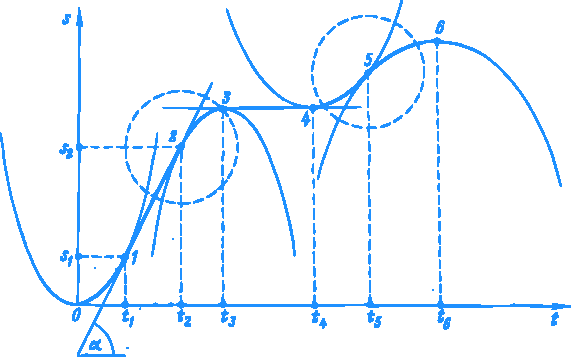
\includegraphics[width=\textwidth]{figures/fig-31.pdf}
\caption{Analysing the concept of instantaneous velocity.}
\label{fig-31}
\end{figure}

\athr Consider a graph of distance covered by a body plotted as a function of time, that is, the graph of the function $s = s (t)$. This graph is shown in \fig{fig-31} by a solid line. Note that in physics one typically uses the same symbol to denote both a function and its values (in this case we use the symbol $s$).

\rdr The figure also shows several thin lines.

\athr The thin lines (parabolas: and straight lines) are shown only to indicate how the graph of $s = s (t)$ was plotted. This graph is thus composed of ``pieces'' of parabolas and straight lines. For instance, for the time interval from 0 to $t_{1}$ the graph is represented by a ``piece'' of the extreme left-hand parabola (portion 0-1 of the graph). Please recall the formula for the distance covered in a uniformly accelerated motion with zero initial velocity.

\rdr This formula is 
\begin{equation}%
s (t) =\dfrac{at^{2}}{2}
\label{uniform-dist}
%eq-1
\end{equation}
 where $a$ is acceleration. 

\athr And the extreme left-hand parabola is the
graph of the function represented by your formula. 

\rdr So for the time interval from 0 to $t_{1}$ the body moves at a constant acceleration. 

\athr Exactly. 

\rdr I see. For the time interval from $t_{1}$ to $t_{2}$ the
body moves uniformly (portion 1-2 of the graph is a straight line); from $t_{2}$ to $t_{3}$ the body moves at a constant deceleration (the graph is an inverse parabola); from $t_{3}$ to $t_{4}$ the body is not moving at all; from $t_{4}$ to $t_{5}$ it moves at a constant acceleration, and from $t_{5}$ to $t_{6}$ it moves at a constant deceleration.

\athr Precisely so. Now let us consider the graph of the function $s (t)$ shown in \fig{fig-31} from a purely mathematical standpoint. Let us pose the following question: How strongly do the values of the function change in response
to the value of its argument $t$ in different portions of the graph?

\rdr In portion 3-4 the values of the function $s (t)$ do not change at all, while in other portions they do. A slower rate of change of the function is observed in the vicinity	of	points	0,	3,	4,	and	 6;	a	faster	rate of change is observed in the vicinity of points 1, 2, and 5. As a matter of fact, the rate of change is equally fast throughout portion 1-2.

\begin{figure}[!ht]%[13]{r}{0.5\textwidth}
\centering
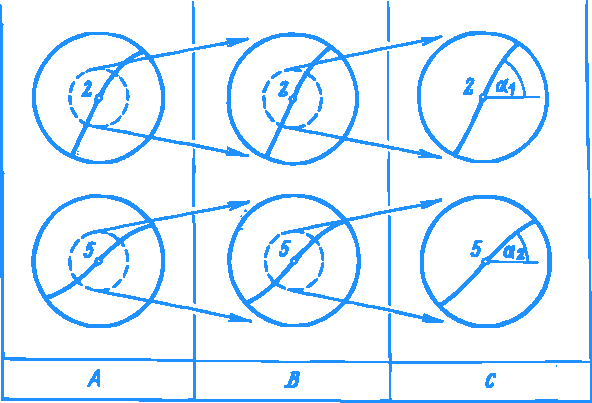
\includegraphics[width=\textwidth]{figures/fig-32.pdf}
\caption{Analysing the concept of instantaneous velocity mathematically.}
\label{fig-32}
\end{figure}

\athr You are a keen observer. And where do you think the rate of change is faster, at point 2 or at point 5? 

\rdr Of course, at point 2. Here the graph of the function has a much steeper slope than at point 5.	

\athr Let us turn to \fig{fig-32}. Here in column $A$ two portions of the graph of the function $s (t)$ are shown separately, namely, those in the vicinity of points 2 and 5 (in \fig{fig-31} these portions are identified by dash circles). In column $B$ the portions of the graph close to points 2 and 5 are shown again, but this time with a two-fold increase in scale. Column $C$ shows the result of another two-fold scale increase. Obviously, as the scale increases, the curvature of the graph $s (t)$ becomes less noticeable. We may say that the graph has a property of ``linearity on a small scale'', which enables us to consider the slope of the graph \emph{at a specific point}. In \fig{fig-32} (in column $C$) it is shown that the slope of the graph at point 2 is ($\alpha_{1}$ (the slope is measured relative to the $t$-axis), while the slope at point 5 is $\alpha_{2}$, and
clearly $\alpha_{2} < \alpha_{1}$.

Denote the slope of the curve $s (t)$ at the moment $t$ by $\alpha (t)$. Then $\tan \alpha (t)$ is said to be the rate of change of the function $s (t)$ at the moment $t$, or simply the instantaneous velocity.

\rdr But why tangent?

\athr You immediately come to it by considering portion 1-2 of the graph in \fig{fig-31}. This portion represents a uniform motion of the body, the rate of change of $s (t)$ being identical at all points. Obviously, it equals the
average velocity during the time interval $t_{2} -	t_{1}$ , which is 
\begin{equation*}%
\frac{s_{2}-s_{1}}{t_{2} - t_{1}} = \tan \alpha
\end{equation*}

\rdr In \fig{fig-32} you have demonstrated a ``straightening'' of the graph by increasing its scale. But this straightening is only \emph{approximate}. Why have you stopped at a mere four-fold scale increase?

\athr We can get rid of this approximation and formulate a more rigorous definition of a slope at a point. To be more specific, we consider a segment of the graph $s (t)$ close to point 5. In this segment we select an arbitrary point $B$ and draw a secant through points 5 and B (\fig{fig-33}). Next, on the same graph between points 5 and $B$ we select an arbitrary point $C$ and draw a new secant $5C$. Further, we select an arbitrary point $D$ in the segment between 5
and $C$ and draw a new secant $5D$. We may continue this process infinitely long and, as a result, we obtain a sequence of secants which converges to a certain straight line (line $5A$ in \fig{fig-33}). This straight line is said to be tangent to the curve at point 5. \emph{The slope of the tangent is said to be the slope of the graph at a given point.}
\begin{figure}[!ht]%[13]{r}{0.5\textwidth}
\centering
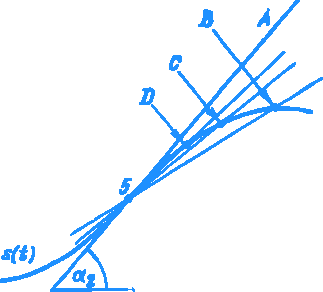
\includegraphics[width=0.5\textwidth]{figures/fig-33.pdf}
\caption{Analysing the concept of instantaneous velocity mathematically.}
\label{fig-33}
\end{figure}

\rdr If I understand you correctly we are now in a position to formulate strictly the answer to the question about the instantaneous velocity.

\athr Try to do it, then.

\rdr The instantaneous velocity of a body at a moment of time $t$ is the rate of change of $s (t)$ at the moment $t$. \emph{Numerically it is equal to the tangent of the slope of the tangent line to the graph of the function $s (t)$ at the moment $t$.}

\athr Very good. But you should have mentioned that $s(t)$ expresses the distance covered by the body as a function of time.

\rdr This is true, my definition of the instantaneous velocity is tied to the \emph{graph} of $s (t)$. What if the function $s (t)$ is not defined graphically?

\athr Anyway, a graph for $s (t)$ always exists. The only ``inconvenience'' in your definition is that it is necessary to take into account the scale of units on the coordinate axes. If the unit of time (on the $t$-axis) and the unit of length (on the $s$-axis) are represented by segments of identical length, the instantaneous velocity at time $t$ is
\begin{equation*}%
\tan \alpha (t) \, \dfrac{\text{unit of length}}{\text{unit of time}}
\end{equation*}
If, however, the segment representing one unit of length is $n$ times greater than the segment representing one unit of time, the instantaneous velocity is
\begin{equation*}%
\frac{1}{n} \, \tan \alpha (t) \, \dfrac{\text{unit of length}}{\text{unit of time}}
\end{equation*}
This ``inconvenience'', however, has no principal significance. But it is also possible to formulate a definition of the instantaneous velocity in a form free of graphic images.

Look at \fig{fig-34} which carries \fig{fig-33} one step further.
\begin{figure}[!ht]%[13]{r}{0.5\textwidth}
\centering
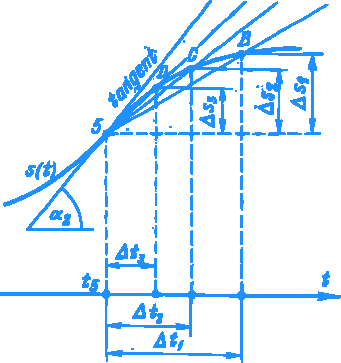
\includegraphics[width=0.5\textwidth]{figures/fig-34.pdf}
\caption{Analysing the concept of instantaneous velocity mathematically.}
\label{fig-34}
\end{figure}

\fig{fig-34} shows that the slope of the secant $5B$ is a ratio $\dfrac{\Delta s_{1}}{\Delta t_{1}}$. In other words, this is the average velocity for the time interval from $t_{5}$ to $t_{5} + \Delta t_{1}$. The slope of the secant $5C $is  $\dfrac{\Delta s_{2}}{\Delta t_{2}}$ that is, the average velocity for the time interval from  $t_{5}$ to  $t_{5} + \Delta t_{2} \,\, (\Delta t_{2} < \Delta t_{1})$. The slope of the secant $5D$ is $\dfrac{\Delta s_{3}}{\Delta t_{3}}$ that is, the average velocity for the time interval from $t_{5}$ to  $t_{5} + \Delta t_{3} \,\, (\Delta t_{3} < \Delta t_{2})$ , etc. Thus, a sequence of the secants converging to the tangent line (drawn at point 5 of the graph $s (t)$) corresponds to a sequence of the average velocities converging to the slope $\alpha_{2}$ of the tangent line, that is, to the value of the instantaneous velocity at the time moment $t_{5}$.

\rdr It comes out that the \emph{instantaneous velocity is the limit of a sequence of average velocities}.

\athr Precisely. The instantaneous velocity is in fact the limit of a sequence of average velocities, provided that the time interval over which the averaging is made tends to zero converging to the moment of time $t$ (viz., $t_{5}$ in \fig{fig-34}).

Now let us formulate the definition in a more rigorous manner. What we want to define is the instantaneous velocity of a body at a moment of time $t$. Consider an arbitrary time interval from $t$ to $t + \Delta t_{1}$. The distance covered by the body during this interval is $\Delta s_{1}$. The average velocity of the body during this time interval is
\begin{equation*}%
v_{\text{av}}  (t, \, \Delta t_{1}) = \frac{\Delta s_{1}}{\Delta t_{1}} 
\end{equation*}
Next we select a shorter time interval $\delta t_{2}$, from $t$ to $t + \Delta t_{2}, \,\, (\Delta t_{2} < \Delta t_{1})$, during which a distance $\Delta s_{2}$ is covered.  Consequently, the average velocity over $\Delta t_{2}$ is
\begin{equation*}%
v_{\text{av}}  (t, \, \Delta t_{2}) = \frac{\Delta s_{2}}{\Delta t_{2}} 
\end{equation*}
We continue this process of selecting shorter and shorter time intervals starting at the moment of time $t$. As a result, we obtain a sequence of the average velocities
\begin{equation*}%
v_{\text{av}}  (t, \, \Delta t_{1}), \,\, v_{\text{av}}  (t, \, \Delta t_{2}), \,\, v_{\text{av}}  (t, \, \Delta t_{3}), \ldots
\end{equation*}
The limit of this sequence for $ \Delta t \to 0$ is the instantaneous
velocity at the moment of time $t$:
\begin{equation}%
v(t) = \lim\limits_{ \Delta t \to 0} v_{\text{av}}  (t, \, \Delta t)
\label{instant-velocity}
%eq-2
\end{equation}
Taking into account that
\begin{equation*}%
v_{\text{av}}  (t, \, \Delta t) = \frac{s (t + \Delta t) - s(t)}{\Delta t}
\end{equation*}
we rewrite expression \eqref{instant-velocity} in the following form
\begin{equation}%
\boxed{
v(t) = \lim\limits_{ \Delta t \to 0} \frac{s (t + \Delta t) - s(t)}{\Delta t}}
\label{instant-velocity}
%eq-3
\end{equation}
As a result, we can formulate the following definition of the instantaneous velocity.
\begin{mytheo}{Definition}
The instantaneous velocity at a moment of time t is the limit of a sequence of average velocities over time intervals from $t$ to $t + \Delta t$ for $\Delta t \to 0$.
\end{mytheo}

\rdr Now I realize that instead of talking about a sufficiently small time interval $\Delta t $ (I am referring to our talk about the ratio $\dfrac{\Delta s }{\Delta t }$ at the beginning of the dialogue), the argument should have been based on the limit transition for $\Delta t \to 0$. In other words, the instantaneous velocity is not $\dfrac{\Delta s }{\Delta t }$  at a sufficiently small  $\Delta t$ but $\lim\limits_{\Delta t \to 0} \, \dfrac{\Delta s }{\Delta t }$ 

\athr Exactly. The definition formulated above for the instantaneous velocity not only exposes the gist of the concept but gives a rule for its calculation, provided that an analytical expression for $s (t)$ is known. Let us make such a calculation assuming that $s(t)$ is given by expression \eqref{uniform-dist}. 

\rdr We should substitute \eqref{uniform-dist} for \eqref{instant-velocity}. This gives
\begin{equation*}%
v(t) =  \lim\limits_{ \Delta t \to 0} \frac{\dfrac{a (t + \Delta t)^{2}}{2} - \dfrac{a t^{2}}{2}}{\Delta t}
\end{equation*}
\athr Go ahead. Remove the parentheses. 

\rdr This will give
\begin{equation*}%
\begin{split}
v(t) & =  \lim\limits_{ \Delta t \to 0} \frac{a (t^{2} + 2t \Delta t + \Delta t^{2} - t^{2})}{2 \Delta t}\\
& = \lim\limits_{ \Delta t \to 0} \left( at + \frac{\Delta t }{2} \right) \\
& = at
\end{split}
\end{equation*}
We have arrived at a familiar formula for the velocity of
uniformly accelerated motion with zero initial velocity:
\begin{equation}%
\boxed{
v(t) = at}
\label{uniform-velocity}
%eq-4
\end{equation}

\athr You are absolutely right. I must congratulate you: for the first time in your life you have carried the so-called operation of \emph{differentiation}. In other words, you have determined for a given function $s (t)$ its \emph{derivative}, that is, the function $v (t)$.

\rdr Does it mean that the instantaneous velocity is a derivative?

\athr Note that a derivative exists only \emph{with respect to} a known \emph{initial} function. If the initial function is $s (t)$ (path as a function of time), the derivative is the instantaneous velocity.

\begin{figure}[!ht]%[13]{r}{0.5\textwidth}
\centering
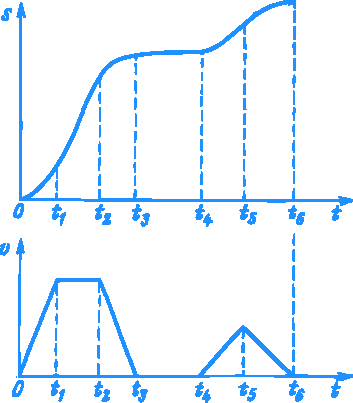
\includegraphics[width=0.6\textwidth]{figures/fig-35.pdf}
\caption{Comparing the graph of a function $s(t)$ and the graph of its rate
of change.}
\label{fig-35}
\end{figure}

Let us return now to the graph $s (t)$ shown in \fig{fig-31}. Our previous arguments and, in particular, relation \eqref{uniform-velocity}, allow us to transform the graph $s (t)$ into a graph of the derivative, that is, the function $v (t)$. A comparison of the two graphs is given in \fig{fig-35}. I recommend that you carefully analyze \fig{fig-35}, interpreting it as a comparison of the graph of a function $s (t)$ and the graph of its rate of change.}